\documentclass{standalone}
\usepackage{tikz, fkmath}
\begin{document}
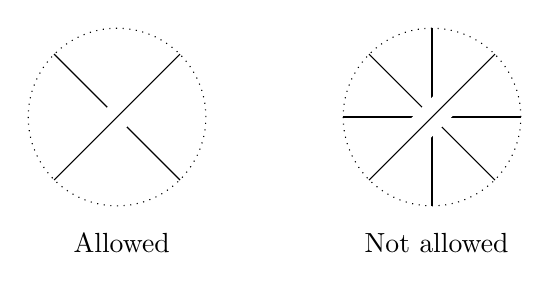
\begin{tikzpicture}[scale=.8]
  \begin{scope}[xshift=-2.5cm]
    \draw (-1,1) -- (1,-1);
    \draw[white, line width=10pt] (1,1) -- (-1,-1);
    \draw (1,1) -- (-1,-1);
    \node () at (0,-2) {\cmark\ Allowed};
    \draw[dotted] (0,0) circle (1.41);
  \end{scope}

  \begin{scope}[xshift=2.5cm]
    \draw (-1.41, 0) -- (1.41, 0);
    \draw (0,-1.41) -- (0,1.41);
    \draw (-1, 1) -- (1,-1);
    \draw[white, line width=10pt] (1, 1) -- (-1,-1);
    \draw (1, 1) -- (-1,-1);
    \node () at (0,-2) {\xmark\ Not allowed};
    \draw[dotted] (0,0) circle (1.41);
  \end{scope}
\end{tikzpicture}
\end{document}
